\subsection{Performances Studies based on Phase 1 Pixel Detector}

\subsubsection{Developed tools: summarizing the work we are doing to have the needed simulation tools to perform our studies}

\vspace{0.5 cm}
\textbf{The L1PixelTrigger Analyzer}

An EDAnalyzer is a module in the \texttt{CMSSW} framework that allows to extract information from datasets
containing simulated or collision data. The extracted information is usually saved in files browsable by ROOT,
and organized in a TTree structure. In our particular case, the TTree was called \textit{NtupleMaker} and it
contais several branches documented below.

Previous analyzers were useful guidelines to build the \textit{L1PixelTrigger}, between them are the
\textit{PixelTree} provided by the Tracker Detector Performance Group (DPG~\cite{ref:DPG}), and the \textit{TrackTriggerStudy}
provided by the Track Trigger Integration (TTI~\cite{ref:TTI}) group.

\vspace{0.5 cm}
\textbf{Code and Documentation}

The \textit{L1PixelTrigger} analyzer was developed in \texttt{CMSSW\_6\_1\_2\_SLHC6\_patch1}, with the routine
{\it mkedanlzr L1PixelTrigger}. The source code, named {\it L1PixelTrigger.cc}, is available at

{\it https://github.com/jruizvar/pixel-analysis/}. 

The collections retrieved by the analyzer are:

\begin{itemize}
\item \textbf{\textit{PileupSummaryInfo}}: Provides the number of interaction per bunch crossing. This collection
stores sixteen bunch crossings (12 early, one in-time, three late). To retrieve the pileup distribution, we have
to loop into the collection and use the method \texttt{getPU\_NumInteractions()} for each bunch. The associated
branch in the ROOT file is called  {\it pileup}.
\item \textbf{\textit{BeamSpot}}: Provides the position and error of the beam spot.  The associated branches are
{\it beamSpotX0}, {\it beamSpotX0Error}, {\it beamSpotY0}, {\it beamSpotY0Error},
{\it beamSpotZ0}, and {\it beamSpotZ0Error}. This collection also provides details about the beam. The width and
error in the transverse plane are given by {\it beamWidthX}, {\it beamWidthXError}, {\it beamWidthY}, and
{\it beamWidthYError}. The spread and error along the Z direction is given by {\it beamSigmaZ}, and
{\it beamSigmaZError}.
\item \textbf{\textit{GenParticleCollection}}: Provides information of the event at the generator level. The
multiplicity of \textit{GenParticles} corresponds to the size of the collection, and is stored in the branch
{\it genPartN}. Relevant information is stored in the branches {\it genPartEt}, {\it genPartPt},
{\it genPartEta}, {\it genPartPhi}, {\it genPartCharge}, and {\it genPartId}. The \textit{GenParticleCollection}
does not include the underlying particles in samples with pileup. 
\item \textbf{\textit{L1EmParticleCollection}}: Provides information of the event as measured by the electromagnetic
calorimeter. The size of the collection is stored in the branch {\it egN}.
Relevant information is stored in the branches {\it egE, egEt, egEta, egPhi}, and \textit{egCharge}. The method
\texttt{getCalorimeterPosition()} taken from the \textit{TrackTriggerStudy} analyzer, is used to translate from
cylindrical to cartesian coordinates. The output of this method is stored in the branches {\it egGx, egGy, egGz}
and corresponds to the global position in the calorimeter.
\item \textbf{\textit{SiPixelRecHitCollection}}: Provides information of the event as measured by the pixel detector.
The multiplicity of reconstructed hits in the barrel is store in the branch {\it bHitN}. The global position is
stored in the branches {\it bHitGx, bHitGy, bHitGz}. Relevant branches associated with the pixel barrel are
{\it bHitLayer, bHitLadder, bHitModule}. The cluster size is stored in the branch {\it bClSize}. The multiplicity of
reconstructed hits in the endcap is store in the branch {\it fHitN}. The global position is stored in the branches
{\it fHitGx, fHitGy, fHitGz}. Relevant branches associated with the pixel endcap are {\it fHitDisk, fHitBlade,
fHitModule}. The cluster size is stored in the branch {\it fClSize}.
\end{itemize}

\vspace{0.5 cm}
\textbf{Simulation Tools}

Before starting the production of the TTree structure, based on the \textit{L1PixelTrigger} analyzer as described
above, there are two mandatory steps.
\begin{itemize}
\item A sample of electron-gun is produced in a first step. Here, one electron per event is produced in generator
  level together with the {\it GenParticles} collection, and the deposities of energy in the detector components
  are simulated by Geant4~\cite{Agostinelli:2002hh}.
\item Using the electron-gun samples as input, the second step takes place, where the deposities of energy are
  transleted into detector signal, and digital signals are converted into a {\texttt{RAW}} format. This is the
  same format provide by the online system.
\end{itemize}

An offical electron-gun sample, with $E_{T}$ between 2 and 50 GeV, is used as input to the second step. Here the
pile up is added to the electron-gun sample. In order to simulate a scenario of 140 pile up, for example, a total of 140
minimum bias are summed to. Table~\ref{tab:gen-sim-minbias} lists the official electron and minimum bias samples.

\begin{table}[!htb]
  \centering
  \scriptsize
  \caption{Official MC samples (\texttt{GEN-SIM} for electron-gun and Minimum Bias) used to create
    \texttt{DIGI-RAW} and \texttt{Ntuple} files.}
  \label{tab:gen-sim-minbias}
  \begin{tabular}{lcl}
    \hline
        {\bf Description} & {\bf Number of Events} & {\bf Official Samples} \\ \hline \hline
        GEN-SIM           & 50K                    & /SingleElectronFlatPt0p2To50/UpgFall13-POSTLS261\_V2-v1/GEN-SIM \\ \hline
        Minimum Bias      & 30M                    & /MinBias\_TuneZ2star\_14TeV-pythia6/UpgFall13-POSTLS261\_V2-v1/GEN-SIM \\ \hline
  \end{tabular}
\end{table}

Output files of the second step have a \texttt{DIGI-RAW} format. Such samples are produced using configuration
files created with a \texttt{CMSSW} tool called {\it cmsDriver}. Table~\ref{tab:digi-raw} provides a list of
{\it datasetpath} for \texttt{CRAB} corresponding to the \texttt{DIGI-RAW} files in four different pile up
scenarios: 0, 35, 70 and 140 pile up. Since outputs are big files --- a total size range from 12 to 400 GB ---
they are produced via \texttt{CRAB}. These files are located at T2\_SPRACE site and each sample of pile up
contains 50 K events.

\begin{table}[!htb]
  \centering
  \scriptsize
  \caption{\texttt{DIGI-RAW} MC samples created from official electron-gun and Minimum Bias MC samples.
    \texttt{CRAB} {\it datasetpaths} are provided for 0, 35, 70 and 140 pile up from top to bottom lines.
    Each sample has 50K events.}
  \label{tab:digi-raw}
  \begin{tabular}{c}
    \hline
        {\bf Data Set Paths} \\ \hline \hline
        /SingleElectronFlatPt0p2To50/adesouza-SingleElectron\_noPileUP\_50K\_DIGI\_RAW\_v6-a49c986a608faae0f4ff11329e2bb83f/USER \\
        /SingleElectronFlatPt0p2To50/adesouza-SingleElectron\_PU35\_50K\_DIGI\_RAW\_v6-61196276663e836a1b830c8b84a619d4/USER \\
        /SingleElectronFlatPt0p2To50/adesouza-SingleElectron\_PU70\_50K\_DIGI\_RAW\_v6-3752475e524a60330e4a83a2952b3625/USER \\
        /SingleElectronFlatPt0p2To50/adesouza-SingleElectron\_PU140\_50K\_DIGI\_RAW\_v6-f74d2f3945f4866a2ea25695b38d79f0/USER \\ \hline
  \end{tabular}
\end{table}

Production of the TTree structure goes in a third step with the full event reconstruction, where the
\texttt{DIGI-RAW} samples are taken as input into configuration files also created via {\it cmsDriver}.
Four different samples, corresponding to each pile up scenario, are produced via \texttt{CRAB}. They are
located in T2\_SPRACE with sizes varying from 24 MB to 22 GB. This is the file path to them:

{\footnotesize /pnfs/sprace.org.br/data/cms/store/user/adesouza/SingleElectronFlatPt0p2To50/MergedNtuples/}.

In the Phase I upgrade, one extra barrel layer and two extra endcap disks are included in the pixel detector.
Figure~\ref{fig:RZ_view_pixel_hits} has a $r-z$ view of this upgraded pixel system, where the pixel hits are
simulated using a sample of single electron-gun. Barrel layers comprise the region of 548.8 mm along $z$ direction,
and with radii from 3 to 16 cm.

\begin{figure}[!htb]
  \centering
  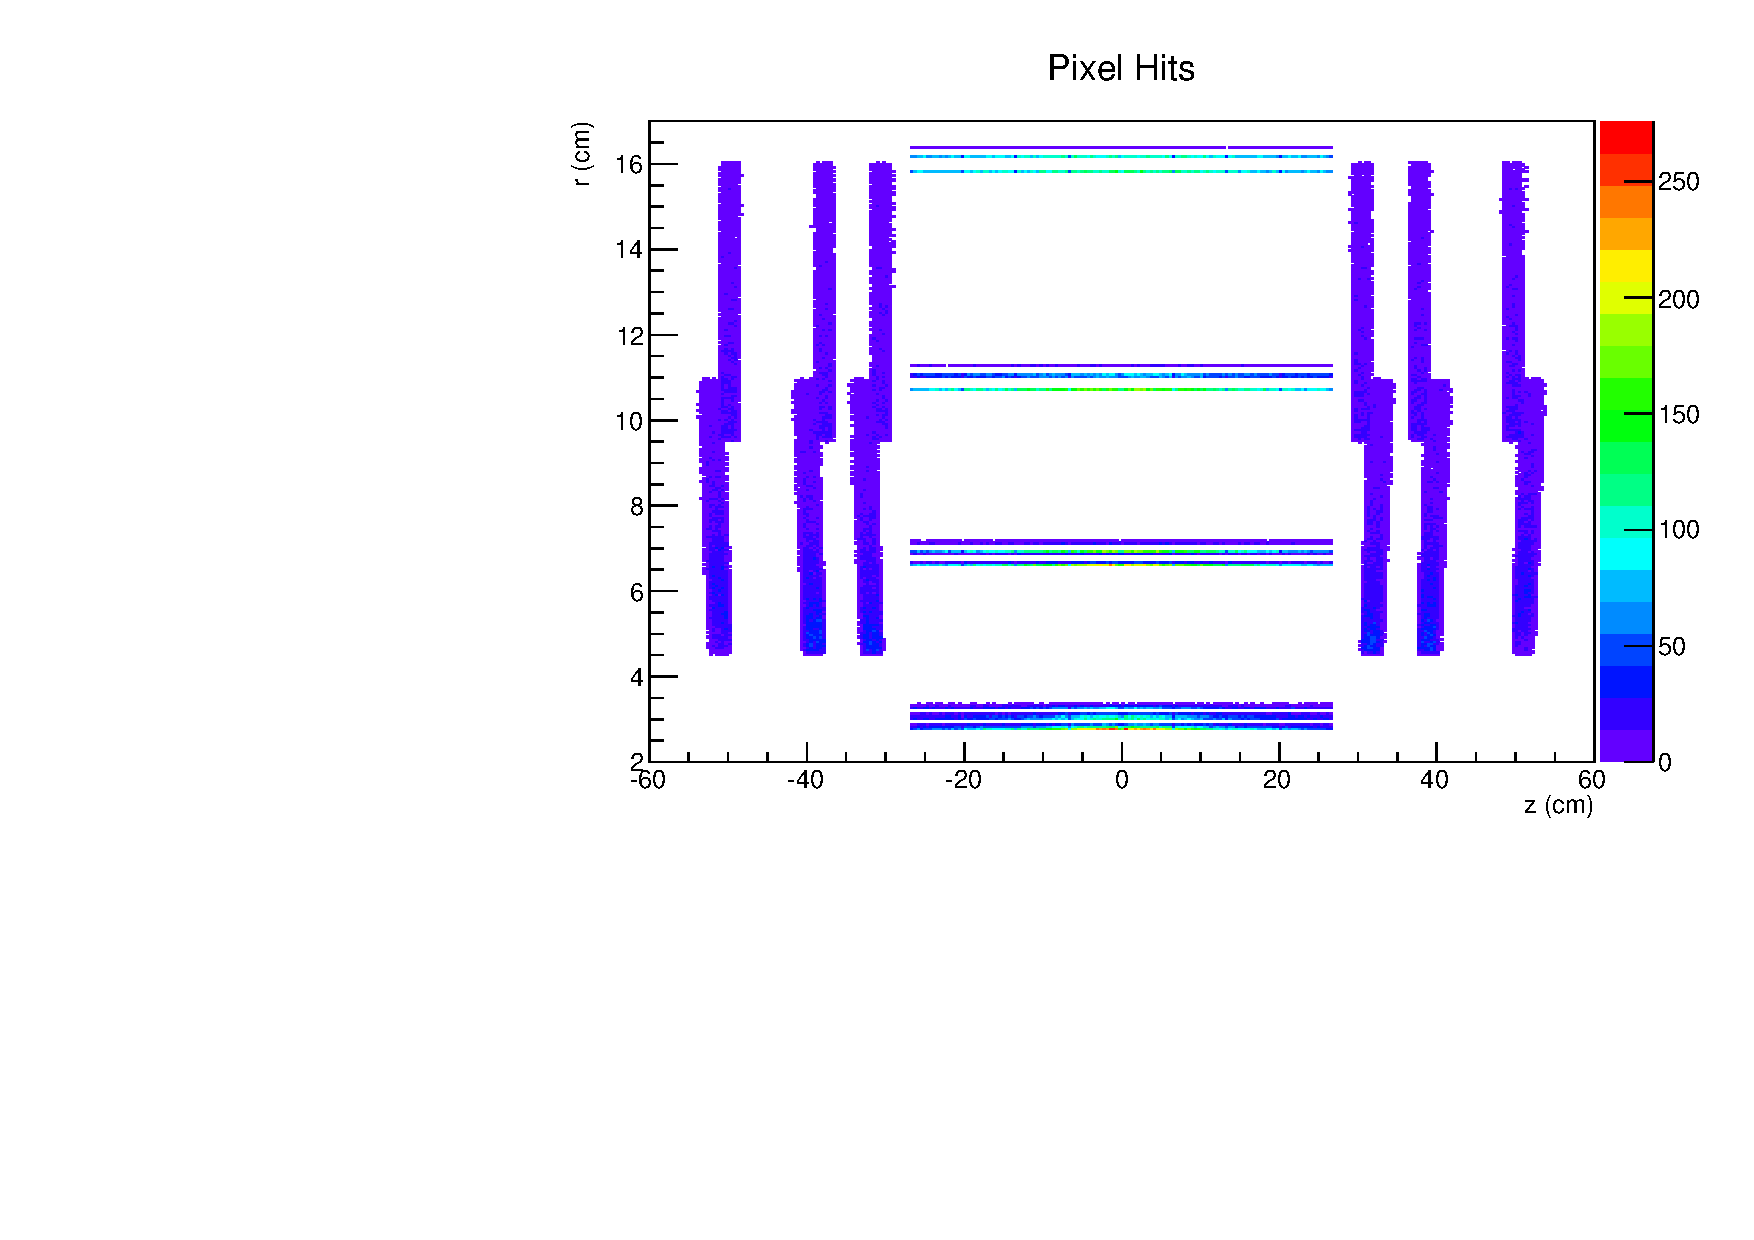
\includegraphics[scale=0.8]{../SimulationTools/RZ_view_pixel_hits_v2.pdf}
  \caption{RZ view of reconstructed hits in the pixel detector.}
  \label{fig:RZ_view_pixel_hits}
\end{figure}

The average number of proton-proton collisions in a bunch crossing depends on the operation characteristics of
the LHC. Figure~\ref{fig:PileUP_4scenarios} shows four different pile up scenarios, following a Poisson
distribution, corresponding to the sample list of single electron-gun produced as described above. In average,
those scenarios have bunch crossings containing 0, 35, 70 and 140 proton-proton collisions.

\begin{figure}[!htb]
  \centering
  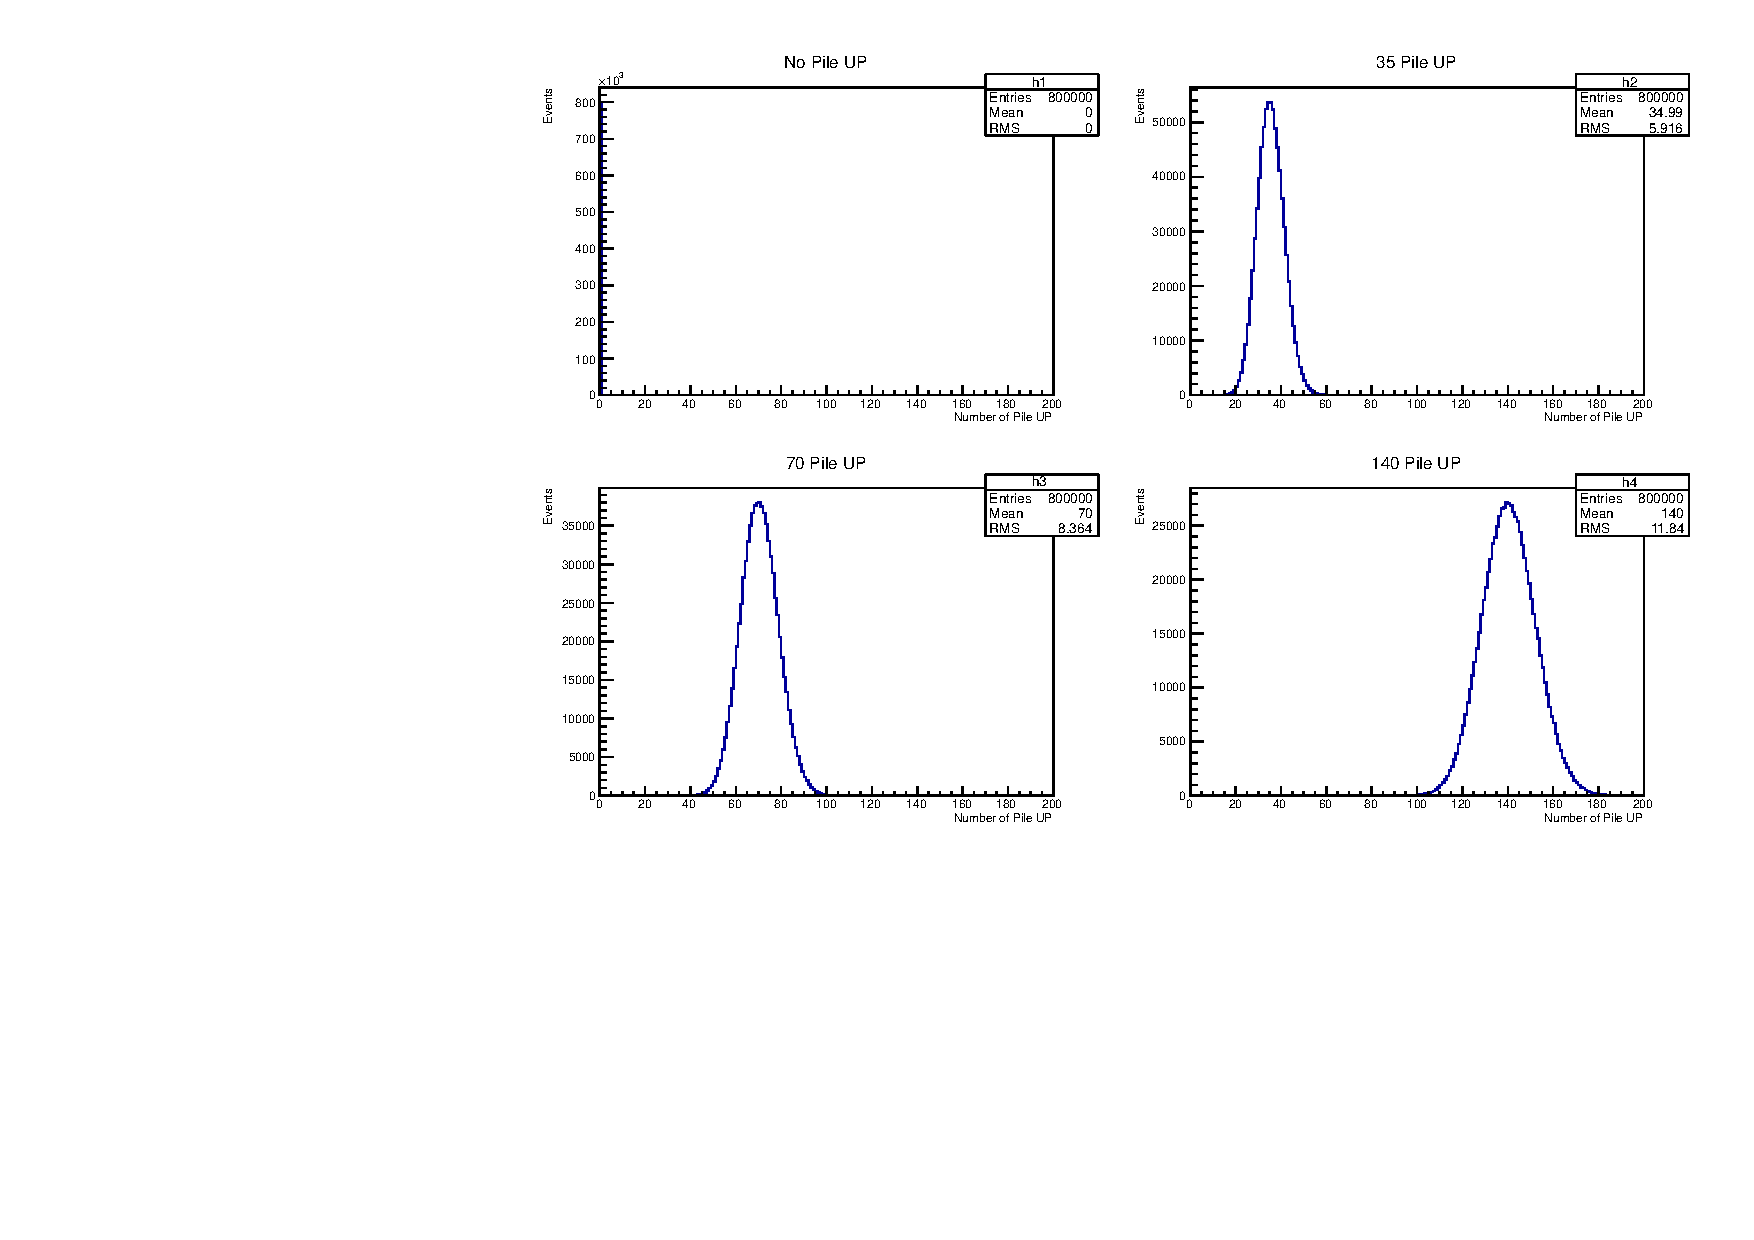
\includegraphics[scale=0.8]{../SimulationTools/PileUP_4scenarios.pdf}
  \caption{Pile up distributions in four different scenarios: zero (top left), 35 (top right), 70 (bottom
    left) and 140 (bottom right) pile up.}
  \label{fig:PileUP_4scenarios}
\end{figure}

The interaction region of proton-proton collisions is also dependent on the characteristics of the LHC operations.
Table~\ref{tab:beam_spot} presents the beam spot positions and its uncertainties for each pile up scenario.

\begin{table}[!htb]
  \centering
  \caption{Beam spot position and associated uncertainty.}
  \label{tab:beam_spot}
  \begin{tabular}{ccc}
  \end{tabular}
\end{table}


\subsubsection{Results on Phase 1 Pixel Detector Performances based on CMSSW6 with emphasis on the effect of increasing luminosity
(JOSE+ANGELO)}

%\begin{itemize}
%\item Results based on CMSSW\_6 with emphasis on the effect of increasing luminosity
%\item and different pixel cluster algorithms.
%\end{itemize}

The amount of particles traveling through the detector is as higher as the number of proton-proton interactions.
Figure~\ref{fig:GenParticles_EtEtaPhi} shows $E_{T}$, $\eta$ and $\phi$ distributions of single electron-gun in
generator level, while Figs.~\ref{fig:L1EM_EtEtaPhi_0PileUP}, \ref{fig:L1EM_EtEtaPhi_35PileUP},
\ref{fig:L1EM_EtEtaPhi_70PileUP} and \ref{fig:L1EM_EtEtaPhi_140PileUP} shows those distributions in case of
0, 35, 70 and 140 pile up, respectively, using the tree structures detailed in the last section.

\begin{figure}[!htb]
  \centering
  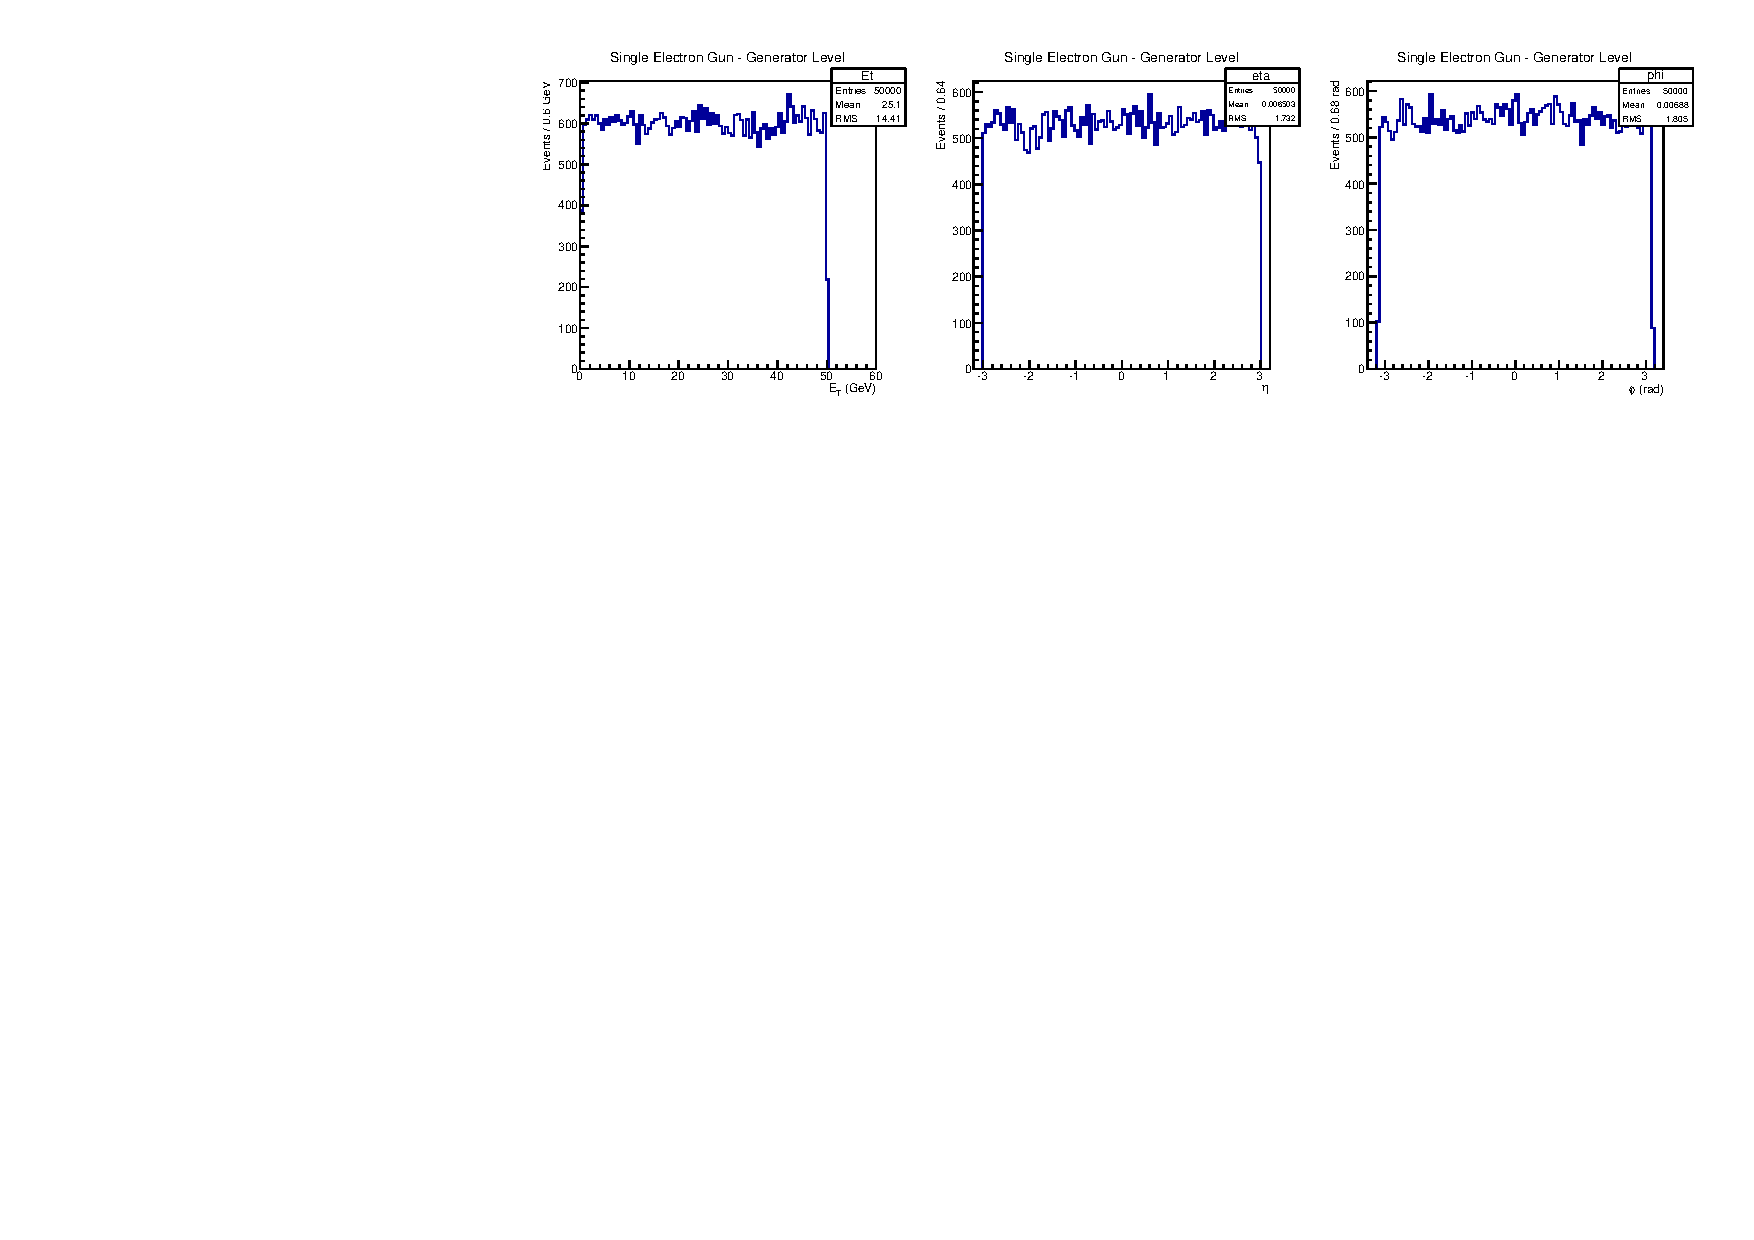
\includegraphics[scale=0.8]{../SimulationTools/GenParticles_EtEtaPhi.pdf}
  \caption{$E_{T}$, $\eta$ and $\phi$ distributions of generated particles (using single electron-gun).}
  \label{fig:GenParticles_EtEtaPhi}
\end{figure}

\begin{figure}[!htb]
  \centering
  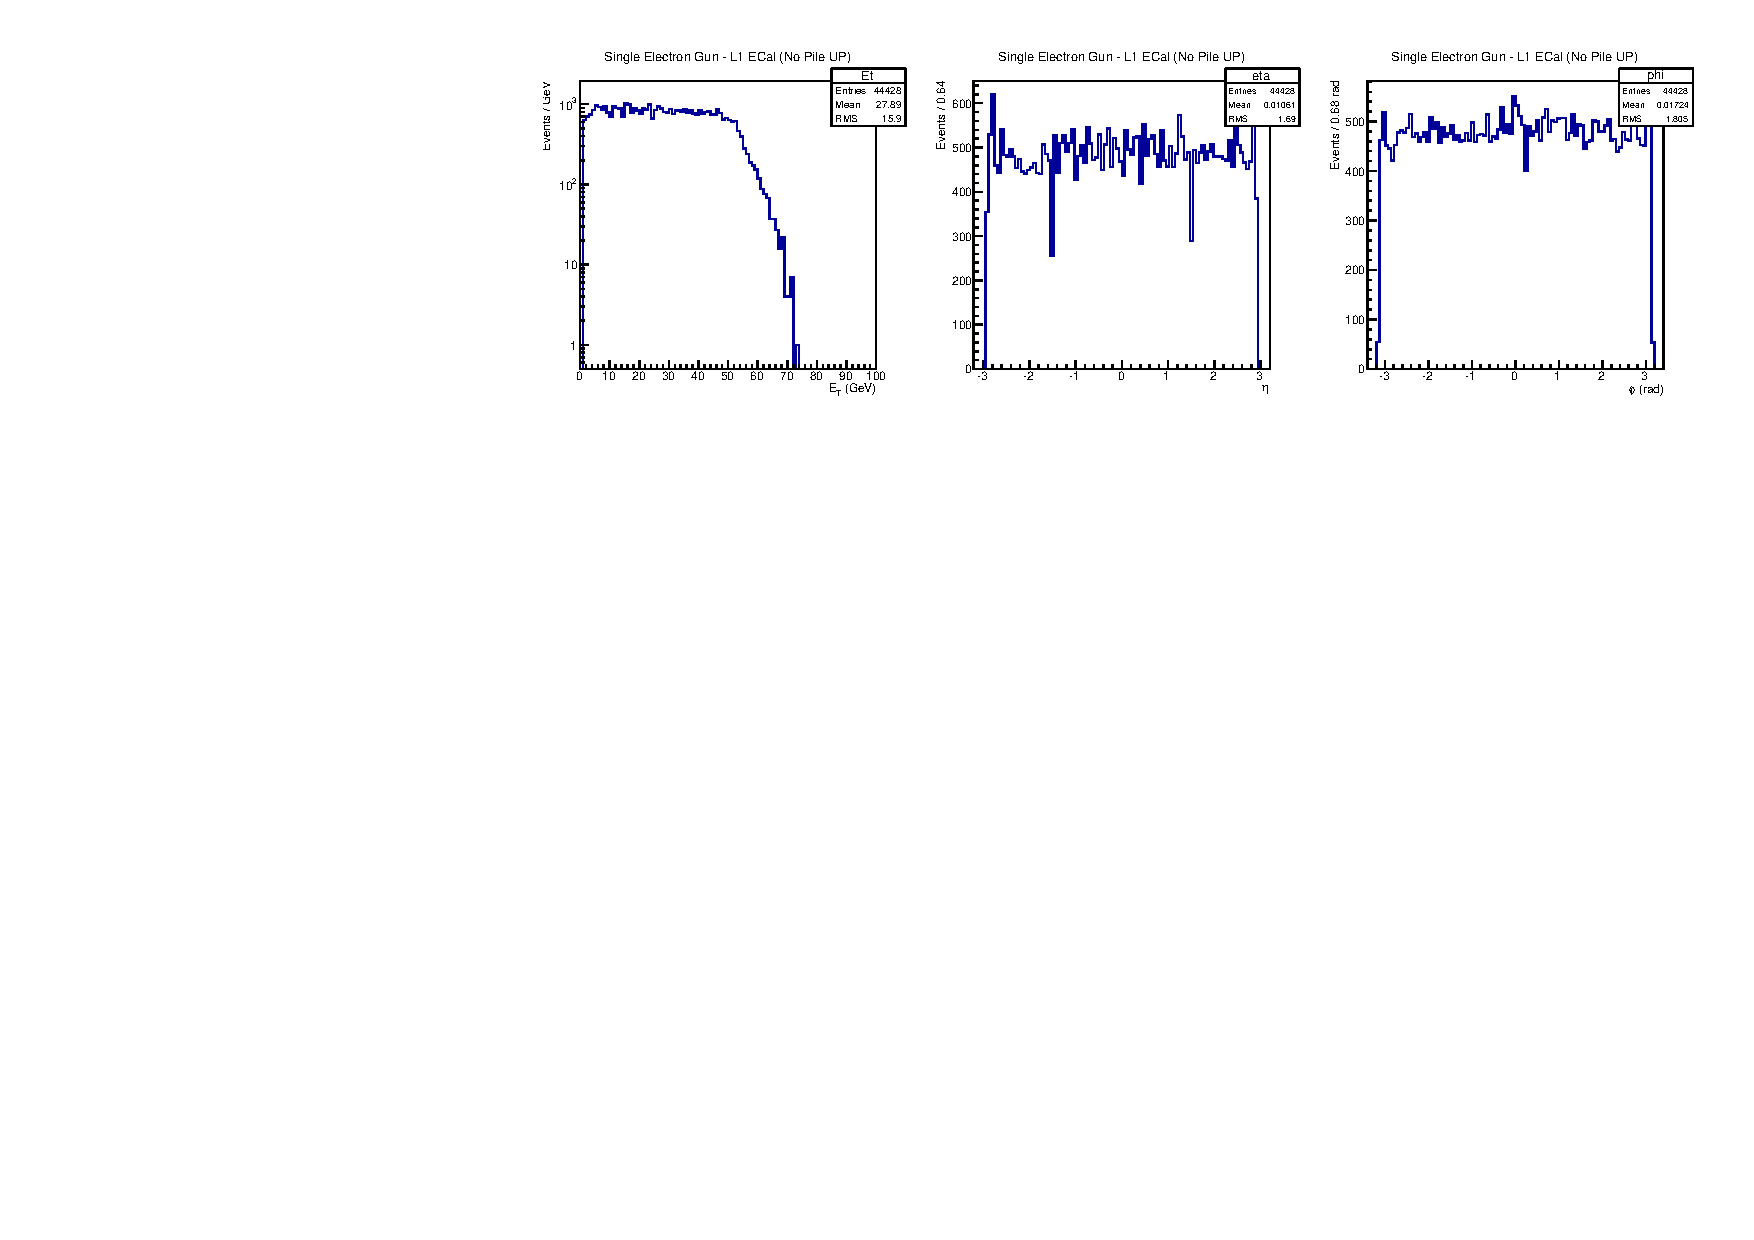
\includegraphics[scale=0.8]{../SimulationTools/L1EM_EtEtaPhi_0PileUP.pdf}
  \caption{$E_{T}$, $\eta$ and $\phi$ distributions of L1EM particles (using single electron-gun) for 0 pile up.}
  \label{fig:L1EM_EtEtaPhi_0PileUP}
\end{figure}

\begin{figure}[!htb]
  \centering
  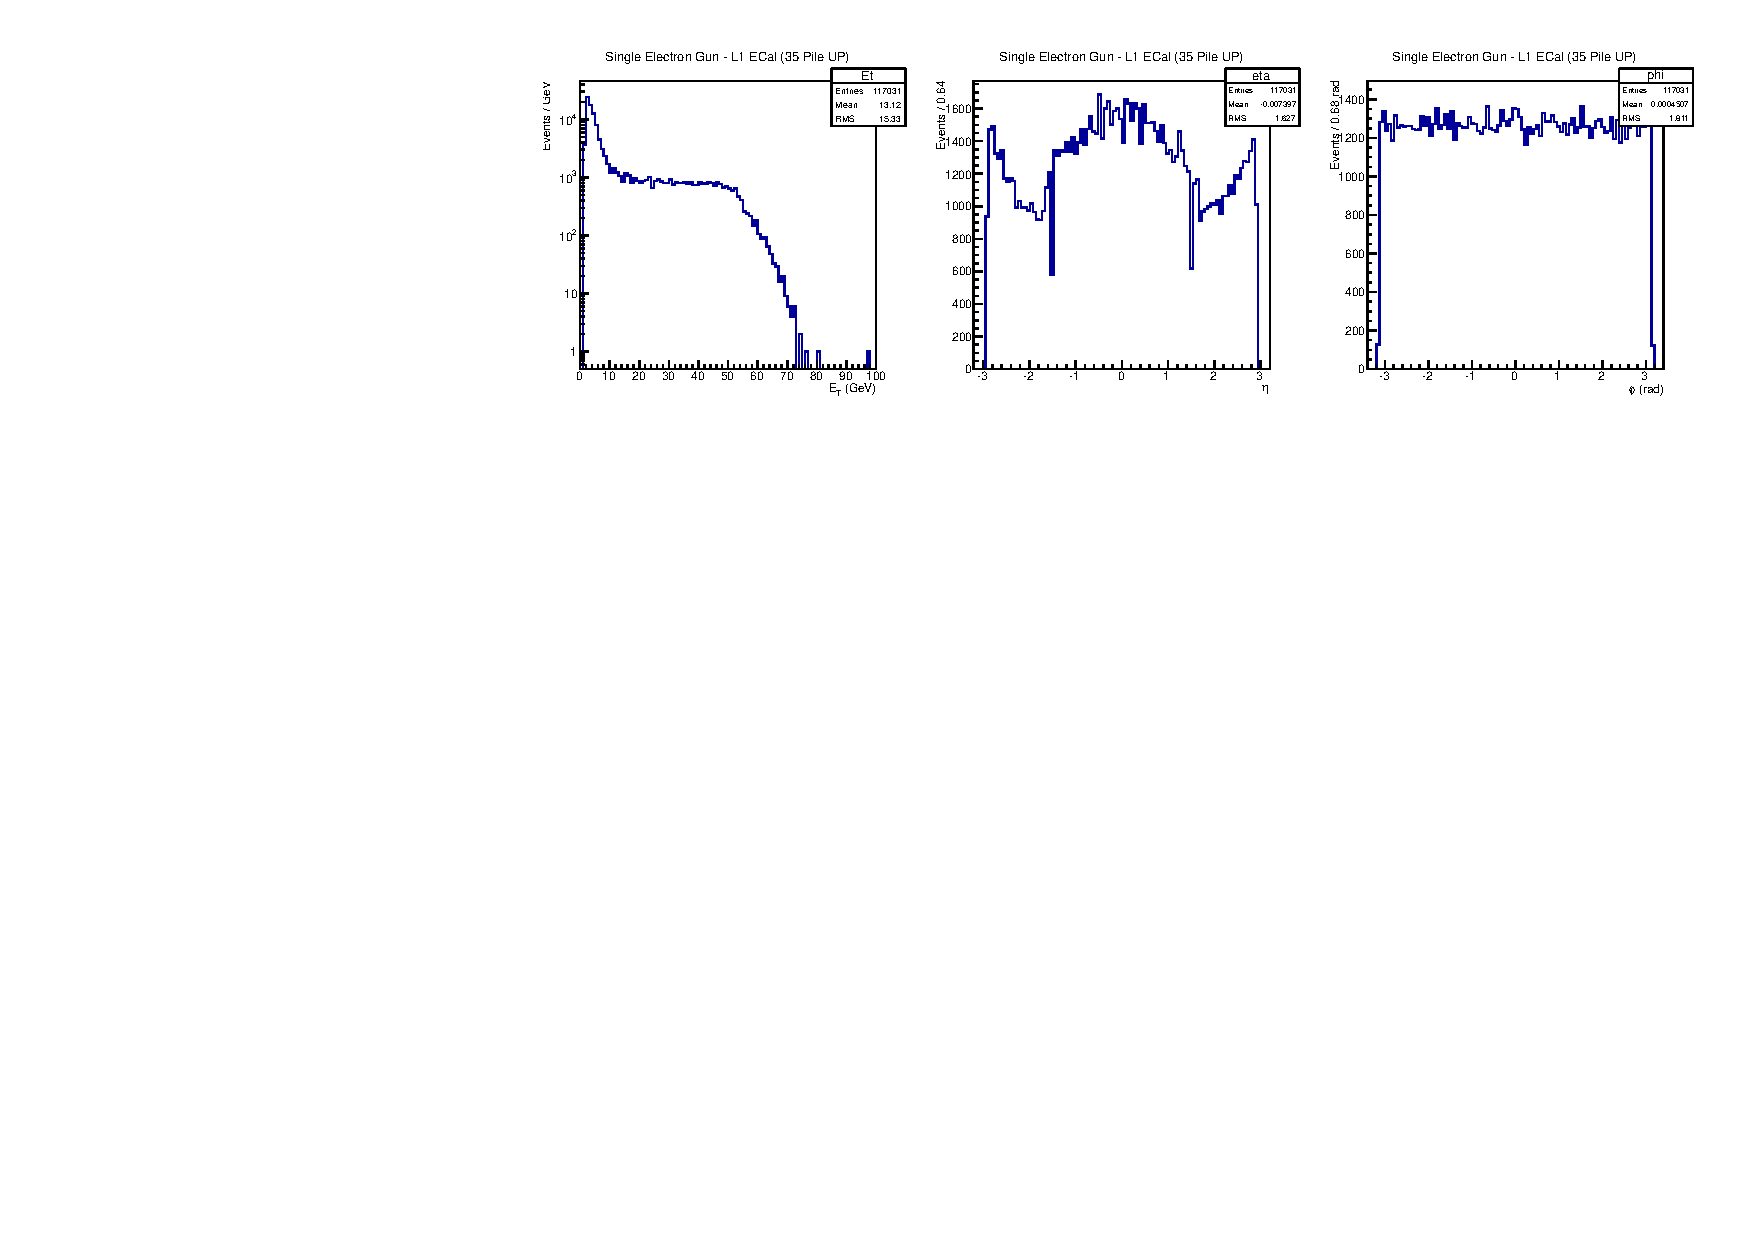
\includegraphics[scale=0.8]{../SimulationTools/L1EM_EtEtaPhi_35PileUP.pdf}
  \caption{$E_{T}$, $\eta$ and $\phi$ distributions of L1EM particles (using single electron-gun) for 35 pile up.}
  \label{fig:L1EM_EtEtaPhi_35PileUP}
\end{figure}

\begin{figure}[!htb]
  \centering
  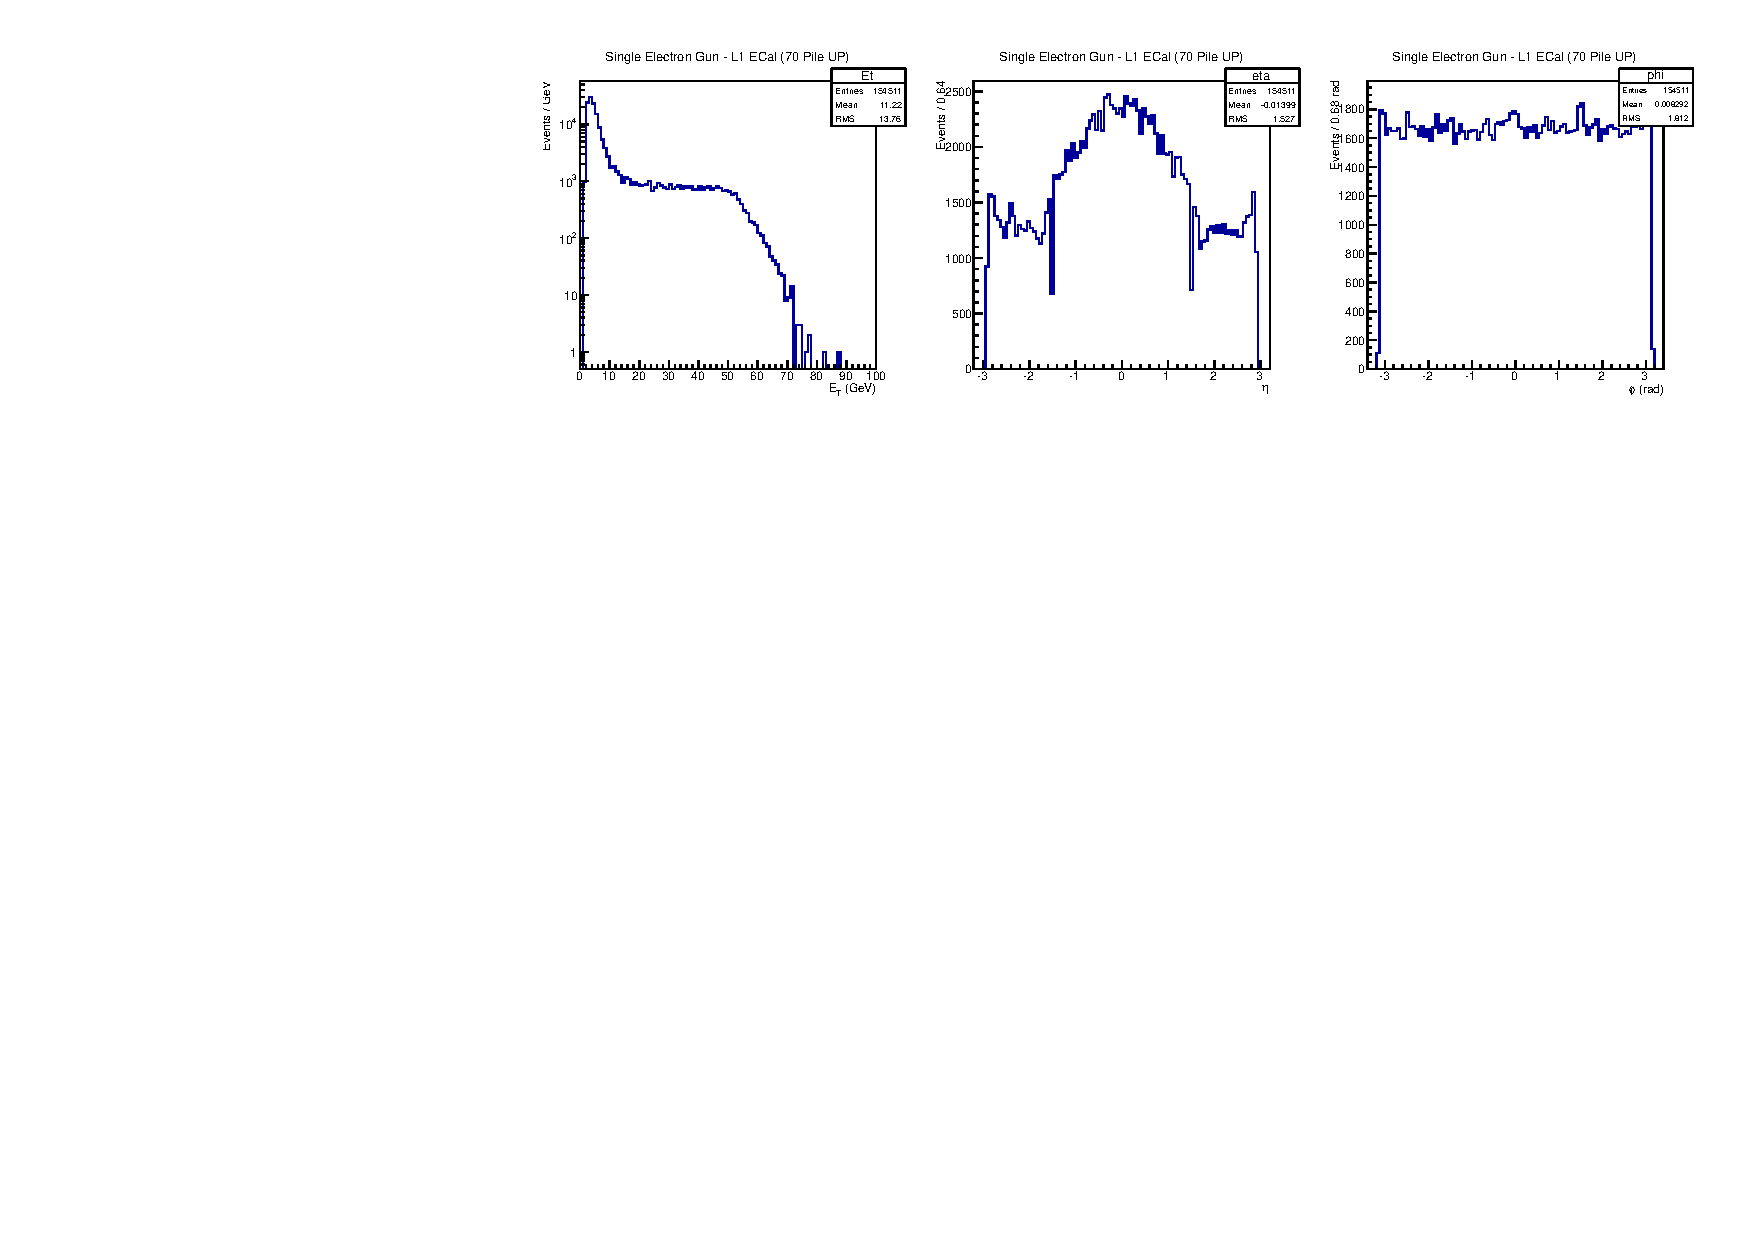
\includegraphics[scale=0.8]{../SimulationTools/L1EM_EtEtaPhi_70PileUP.pdf}
  \caption{$E_{T}$, $\eta$ and $\phi$ distributions of L1EM particles (using single electron-gun) for 70 pile up.}
  \label{fig:L1EM_EtEtaPhi_70PileUP}
\end{figure}

\begin{figure}[!htb]
  \centering
  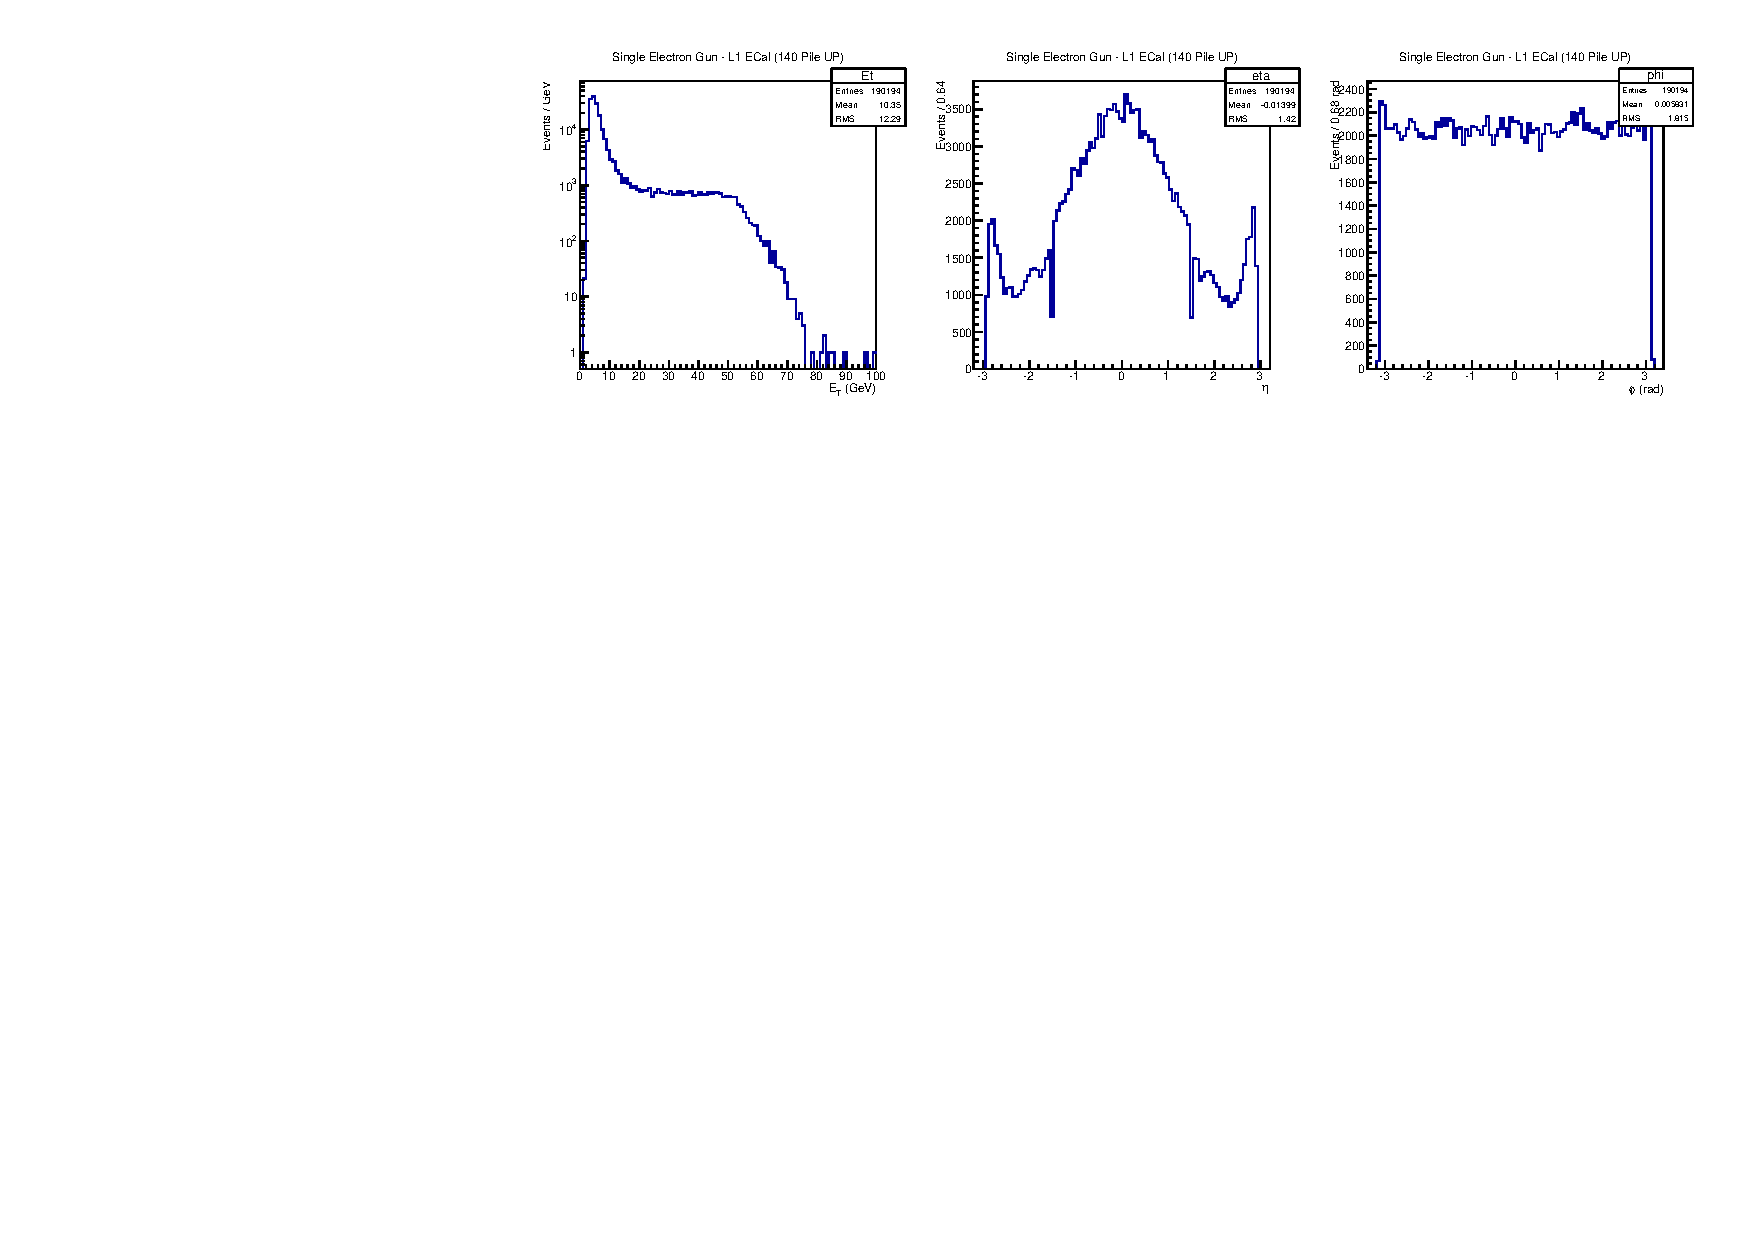
\includegraphics[scale=0.8]{../SimulationTools/L1EM_EtEtaPhi_140PileUP.pdf}
  \caption{$E_{T}$, $\eta$ and $\phi$ distributions of L1EM particles (using single electron-gun) for 140 pile up.}
  \label{fig:L1EM_EtEtaPhi_140PileUP}
\end{figure}

Traveling along the detector, an electron may leave signal in the different components it passes through.
Figure~\ref{fig:Number_of_pixel_clusters} shows a simulation of the number of pixel clusters, per event, in different
barrel layers and disks of the pixel system due to the passage of electrons.

\begin{figure}[!htb]
  \centering
  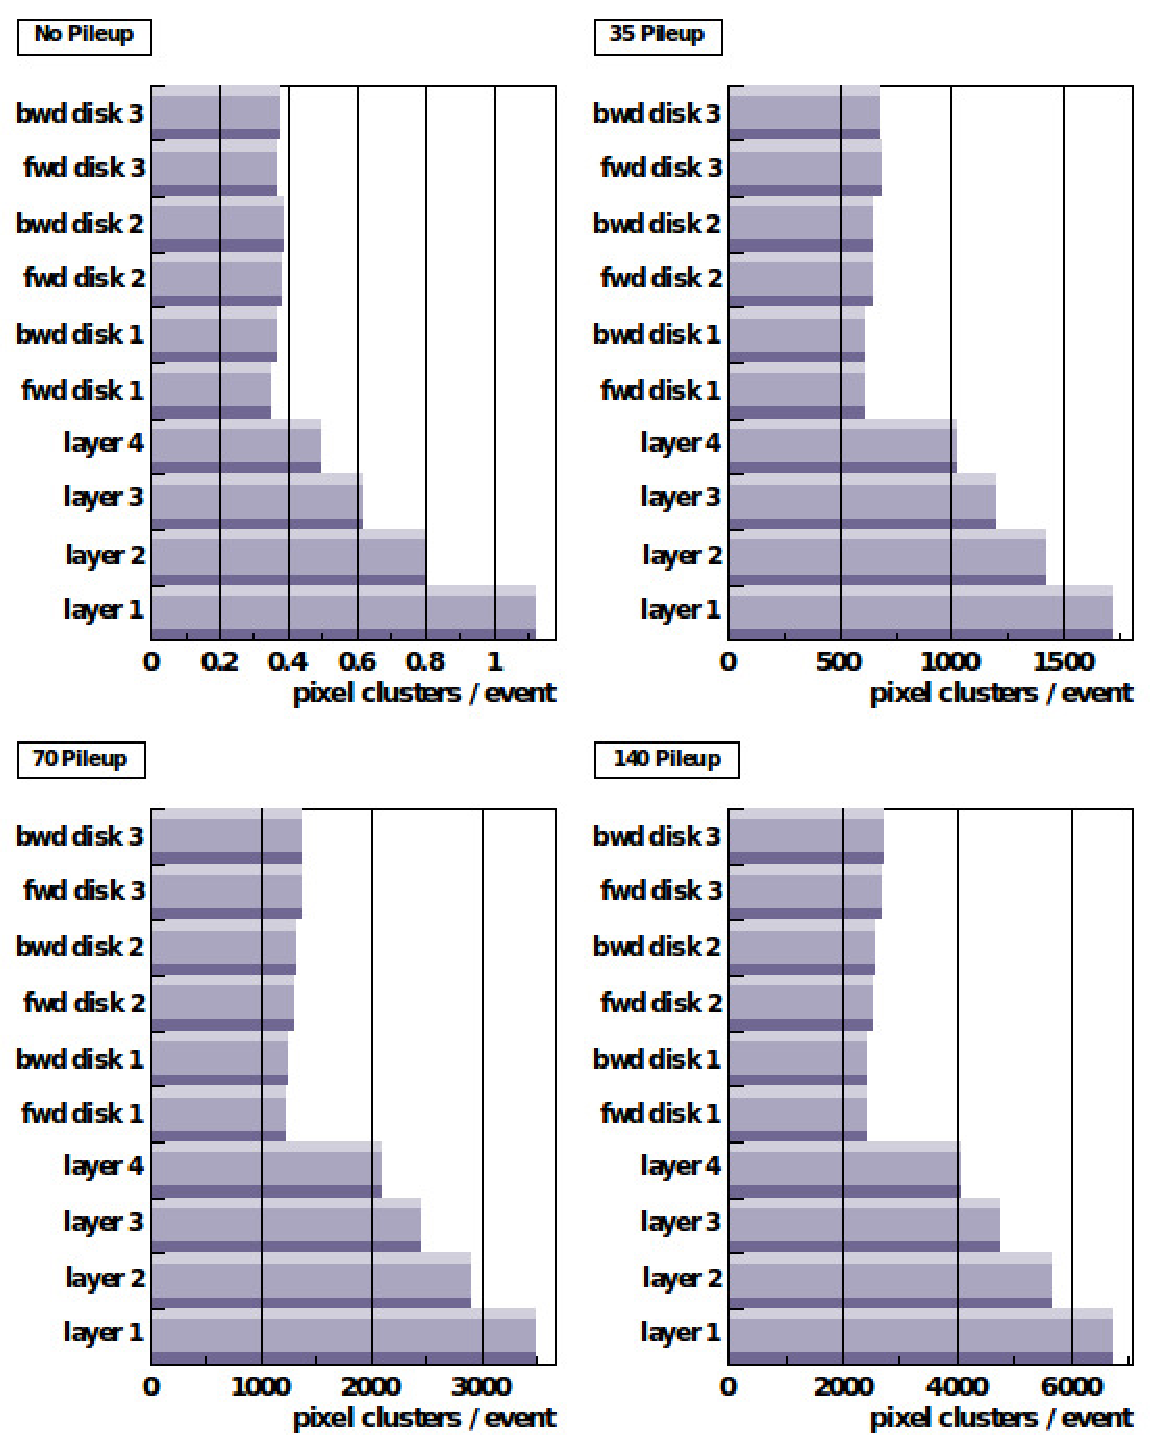
\includegraphics[scale=0.7]{../SimulationTools/Number_of_pixel_clusters.pdf}
  \caption{Number of pixel clusters per event in the different components of the pixel detector left by a single electron.
    Forward $(z>0)$ and backward $(z<0)$ disks are taken separately.}
  %\caption{Pixel clusters and ocuppancies for different pile up scenarios.}
  \label{fig:Number_of_pixel_clusters}
\end{figure}

\clearpage
